\documentclass{article}
\usepackage[T1]{fontenc}
\usepackage[utf8]{inputenc}
\usepackage{indentfirst}
\usepackage{float}
\usepackage{natbib}
\usepackage{graphicx}
\usepackage{grffile}
\usepackage{epsfig}
\usepackage{soul}
\usepackage{pdflscape}
\usepackage{hyperref}
\usepackage[scaled]{helvet}
\renewcommand\familydefault{\sfdefault} 
\usepackage[T1]{fontenc}
\usepackage[a4paper, total={16cm, 25cm}]{geometry}

\title{\textbf{Database's Models}}
\date{April 8, 2020}

\author{\textbf{Nutr.io}}

\begin{document}

\maketitle

\section{Conceptual Model}

\begin{figure}[H]
    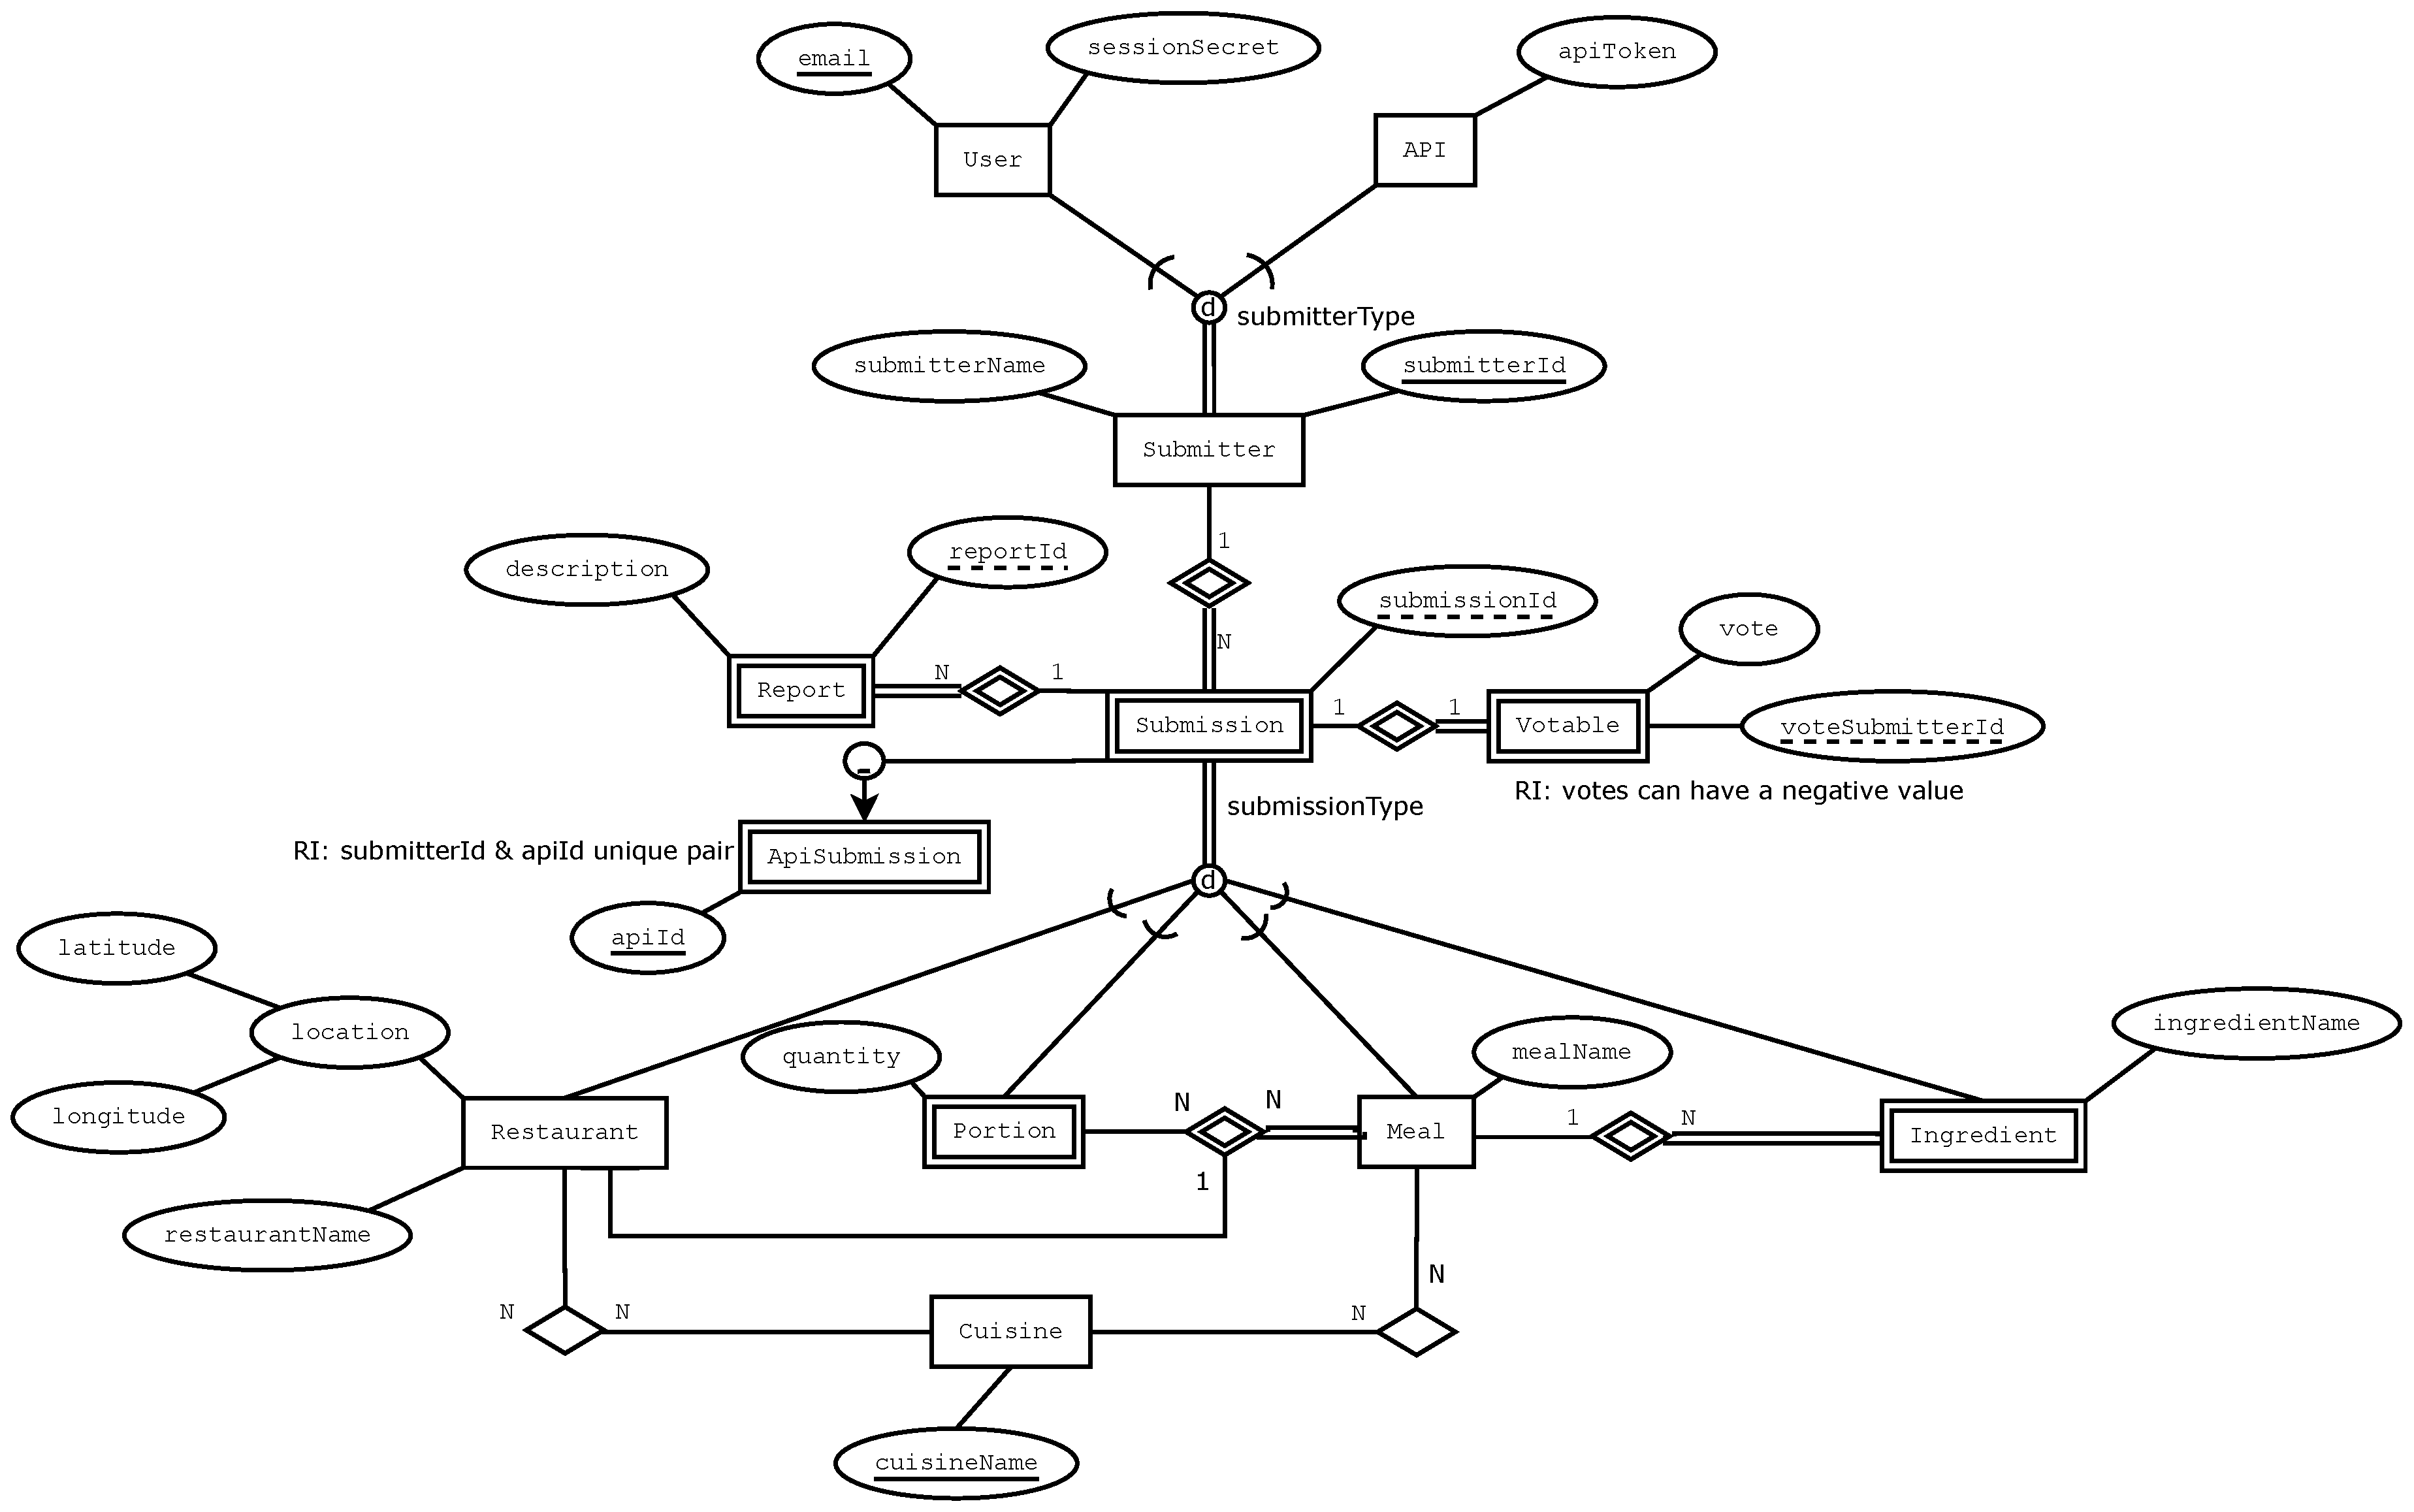
\includegraphics[scale=0.28]{Nutr.io_Database_Diagram.eps}
    \centering 
\end{figure}
\newpage

\section{Relational Model}
    \begin{itemize}
        \item \textbf{Submitter}        
        \begin{itemize}
            \item Attributes: \underline{submitterId}, submitterName, submitterType
            \item Primary Key(s): \underline{submitterId}
            \item Foreign Key(s): -
            \item Not null: submitterName, submitterType
        \end{itemize}

        \item \textbf{User}
        \begin{itemize}
            \item Attributes: \underline{\textit{submitterId}}, \underline{email}, sessionSecret
            \item Primary Key(s): \underline{email}, \underline{\textit{submitterId}}
            \item Foreign Key(s): \underline{\textit{submitterId}} references Submitter
            \item Not null: sessionSecret
        \end{itemize}

        \item \textbf{API}
        \begin{itemize}
            \item Attributes: \underline{\textit{submitterId}}, apiToken
            \item Primary Key(s): \underline{\textit{submitterId}}
            \item Foreign Key(s): \underline{\textit{submitterId}} references Submitter
            \item Not null: apiToken
        \end{itemize}

        \item \textbf{Submission}
        \begin{itemize}
            \item Attributes: \underline{submissionId}, \underline{\textit{submitterId}}, submissionType
            \item Primary Key(s): \underline{\textit{submitterId}}
            \item Foreign Key(s): \underline{\textit{submitterId}} references Submitter
            \item Not null: submissionType
        \end{itemize}

        \item \textbf{ApiSubmission}
        \begin{itemize}
            \item Attributes: \underline{submissionId}, \underline{\textit{submitterId}}, submissionType
            \item Primary Key(s): \underline{\textit{submitterId}}
            \item Foreign Key(s): \underline{\textit{submitterId}} references Submitter
            \item Not null: submissionType
        \end{itemize}

        \item \textbf{Report}
        \begin{itemize}
            \item Attributes: \underline{reportId}, \underline{\textit{submissionId}}, \underline{\textit{submitterId}}, description
            \item Primary Key(s): \underline{reportId}, \underline{\textit{submissionId}},\underline{\textit{submitterId}}
            \item Foreign Key(s): \underline{\textit{submissionId}} references Submission, \underline{\textit{submitterId}} references Submission
            \item Not null: description
        \end{itemize}

        \item \textbf{Votable}
        \begin{itemize}
            \item Attributes: \underline{voteSubmitterId}, \underline{\textit{submissionId}}, \underline{\textit{submitterId}}, vote
            \item Primary Key(s): \underline{voteSubmitterId}, \underline{\textit{submissionId}}, \underline{\textit{submitterId}}
            \item Foreign Key(s): \underline{\textit{submissionId}} references Submission, \underline{\textit{submitterId}} references Submission
            \item Not null: -
        \end{itemize}

        \item \textbf{Restaurant}
        \begin{itemize}
            \item Attributes: \underline{\textit{submissionId}}, \underline{\textit{submitterId}}, restaurantName, latitude, longitude
            \item Primary Key(s): \underline{\textit{submissionId}}, \underline{\textit{submitterId}}
            \item Foreign Key(s): \underline{\textit{submissionId}} references Submission, \underline{\textit{submitterId}} references Submission
            \item Not null: restaurantName, latitude, longitude
        \end{itemize}
    
        \item \textbf{Cuisine}
        \begin{itemize}
            \item Attributes: \underline{cuisineName}
            \item Primary Key(s): \underline{cuisineName}
            \item Foreign Key(s): -
            \item Not null: -
        \end{itemize}

        \item \textbf{Meal}
        \begin{itemize}
            \item Attributes: \underline{\textit{submissionId}}, \underline{\textit{submitterId}}, mealName
            \item Primary Key(s): \underline{\textit{submissionId}}, \underline{\textit{submitterId}}
            \item Foreign Key(s): \underline{\textit{submissionId}} from Submission, \underline{\textit{submitterId}} from Submission
            \item Not null: mealName
        \end{itemize}

        \item \textbf{Portion}
        \begin{itemize}
            \item Attributes: \underline{\textit{submissionId}}, \underline{\textit{submitterId}}, quantity
            \item Primary Key(s): \underline{\textit{submissionId}}, \underline{\textit{submitterId}}
            \item Foreign Key(s):\underline{\textit{submissionId}} from Submission, \underline{\textit{submitterId}} from Submission
            \item Not null: quantity
        \end{itemize}

        \item \textbf{Ingredient}
        \begin{itemize}
            \item Attributes: \underline{\textit{submissionId}}, \underline{\textit{submitterId}}, ingredientName
            \item Primary Key(s): \underline{\textit{submissionId}}, \underline{\textit{submitterId}}
            \item Foreign Key(s): \underline{\textit{submissionId}} from Submission, \underline{\textit{submitterId}} from Submission
            \item Not null: ingredientName
        \end{itemize}

    \end{itemize}
    
\end{document}